\documentclass[../../main.tex]{subfiles}

% 

\begin{document}
\chapter{Spektroskopie záření alfa}

Těžké nabité částice jako třeba $\alpha$ částice interagují s látkou primárně prostřednictvím Coulombické interakce působící mezi jejich kladným nábojem a záporným nábojem orbitálních elektronů atomů absorbátoru. Ačkoliv interakce těžkých nabitých částic s jádry jsou také možné, dochází k nim ale pouze zřídka a za běžných okolností nejsou signifikantní pro odezvu detektorů záření. Charakteristický dosah těžkých nabitých částic je $10^{-5} ~\mathrm{m}$. Trajektorie těžkých nabitých částic v látce je téměř přímková.

Produkty průchodu těžkých nabitých částic absorbátorem jsou buď excitované atomy nebo iontové páry. Každý takový pár je tvořen volným elektronem a odpovídajícím kladným iontem atomu absorbátoru, ze kterého byl odstraněn elektron. Páry iontů mají přirozenou tendenci rekombinovat a znovu utvořit neutrální atom, ovšem v některých typech detektorů je rekombinace potlačena a iontové páry se využívají k vytvoření odezvy detektoru. 

Interakce těžkých nabitých částic:
\begin{itemize}
	\item Elektromagnetická interakce - rozptyl (na elektronech zanedbatelný, na jádrech malá pravděpodobnost), ionizace - hlavní typ interakce
	\item Silná interakce - jaderné reakce, energie vyšší než coulombovská bariéra jader prostředí (pro nízké energie její pravděpodobnost malá a pro detekci je její vliv většinou zanedbatelný)
\end{itemize}
Těžké nabité částice ztrácejí svou kinetickou energii při průchodu látkou následujícími procesy:
\begin{itemize}
	\item excitací a ionizací atomů látky (tzv.  \quotedblbase  elektronové brzdění \textquotedblright - způsobeno  srážkami s atomárními elektrony)
	\item polarizací atomů prostředí (při vysokých energiích)
	\item záchytem elektronu (nábojová výměna) a jaderným brzděním (nastává při malých rychlostech, částice strhává elektrony prostředí)
	\item pružným rozptylem (Coulombickým či jaderným) a jadernými reakcemi
\end{itemize}
Rozptyl má malý vliv, hlavní vliv mají ionizační ztráty - kromě konce mají přímou dráhu a tudíž dobře definovaný dolet. Pokud hovoříme o těžkých nabitých částicích, potom se jedná zejména o $p$, $d$, $t$, $^{3}$H, $\alpha$.

Ztráty kinetické energie těžké nabité částice nakonec vedou k jejímu zastavení v látce. Základními fyzikálními veličinami, které charakterizují průlet nabité částice látkou, jsou lineární brzdná schopnost
\begin{equation}
  S_l = - \left(- \dfrac{dE}{dx} \right) ,
\end{equation}
kde $E$ je kinetická energie, kterou částice ztratí po průletu dráhy $x$, a dosah $R$, jenž udává vzdálenost, jakou částice v látce urazí do svého úplného zastavení. Tyto veličiny závisí jednak na charakteristikách nabité částice (na náboji $Ze$, rychlosti $v$ a hmotnosti $m$), jednak na charakteristikách látky (počtu elektronů $n_e$ v objemové jednotce a na experimentálně stanoveném středním budícím potenciálu $I$)
\begin{equation}
S_l = f(Ze, v, n_e, I), ~~~~~~~~~ R= g (Ze, v, m, n_e, I)
\end{equation}
Střední budící potenciál $I$ představuje geometrický průměr excitačního a ionizačního potenciálu.

Vedle lineární brzdné schopnosti zavádíme také veličinu hmotnostní brzdná schopnost, která je dána vztahem
\begin{equation}
S_m = \left( - \dfrac{1}{\rho} \dfrac{dE}{dx} \right) ,
\end{equation}
kde $\rho$ je hustota látky. Výhoda zavedení hmotnostní brzdné schopnosti je v tom, že se jen málo mění při přechosu k jiné látce (nezávisí na volbě materiálu) a je proto pro praktické výpočty výhodnější. Jiné vyjádření $S_m$ jsou např.
\begin{equation}
s_m \sim \dfrac{1}{\rho} n_e = N_A \dfrac{Z}{A} = N_A \dfrac{1}{1 + \dfrac{N}{Z}},
\end{equation}
kde $n_e$ je počet neutronů, $N_A$ je Avogadrova konstanta. $S_m$ tudíž závisí i na počtu neutronů.

Při ionizaci mohou vzniknout elektrony, které mají dostatečnou energii k tomu, aby samy dále ionizovali. Takové elektrony nazýváme \textbf{delta elektrony}.

\subsection{$\delta$ - elektrony}

Ionizaci způsobenou letící nabitou částicí nazýváme primární ionizací, ne rozdíl od sekundární ionizace způsobené tzv. $\delta$-elektrony (tento termín jako první užil J. J. Thomson).

Tímto termínem nazýváme elektrony, které vznikly při primární ionizaci a získaly takovou kinetickou energii, aby byly schopny při svém letu látkou samy dále ionizovat. Reprezentují tak nepřímý způsob, kterým je možné předat energii nabité částice absorbujícímu médiu. Za normálních podmínek  se totiž většina energetických ztrát nabitých částic děje přes tyto $\delta$-elektrony. Dosah $\delta$-elektronů je vždy menší než dosah původní energetické částice, tudíž jsou další atomy ionizovány v dráze původní částice. 

Celková ionizace nabité částice je dána součtem obou typů interakce.

\subsection{Ztráty energie ionizací - Bethe-Blochova formule}

Výpočet ionizačních a excitačních ztrát provedli Bethe a Bloch, proto následující  vztah (platný pro  nerelativistické částice) nazýváme Bethe-Blochovou formulí
\begin{equation}
\left(- \dfrac{dE}{dx} \right)_{ion} = \left( \dfrac{1}{4 \pi \epsilon_0}\right)^2 \dfrac{4\pi  Z_{ion}^2 e^4}{m_e v^2}  \dfrac{Z}{A} \rho N_A \ln \left( \dfrac{2m_e v^2}{I}\right) ,
\end{equation}
pro vyšší energie musíme zavést relativistické korekce 
\begin{equation}
\left(- \dfrac{dE}{dx} \right)_{ion} = \left( \dfrac{1}{4 \pi \epsilon_0}\right)^2 \dfrac{4\pi  Z_{ion}^2 e^4}{m_e v^2}  \dfrac{Z}{A} \rho N_A \left[ \ln \left( \dfrac{2m_e v^2}{I}\right) - \ln \left( 1 - \dfrac{v^2}{c^2}\right) - \dfrac{v^2}{c^2}\right] ,
\end{equation}
kde $I$ je střední budící potenciál.

K výpočtu bylo použito několik zjednodušení, které je třeba uvést:
\begin{itemize}
	\item Při odvození se vycházelo ze ztráty energie částice při srážce s jedním elektronem. K získání celkové změny energie na jednotku dráhy je třeba ztrátu při jedné srážce násobit hustotou elektronů $n_e = N_A \frac{Z}{A} \rho$ a tuto veličinu následně integrovat přes všechny srážkové parametry mající fyzikální smysl.
	\item Dále bylo uvažováno, že srážku s elektronem je možno popsat klasicky (tj. nekvantově). tento přístup lze použít při dostatečně velkých hybnostech $p$ a dostatečně velkých srážkových parametrech $b$ a musí platit $pb>>\hbar$.
	\item Rychlost dopadající částice je podstatně větší než jsou orbitální rychlosti atomárních elektronů, tj. jde prakticky o rozptyl částice na klidném elektronu.
	\item Elektrony jsou považovány za volné, tj. zanedbává se jejich energie vazby v atomech.
\end{itemize}

\begin{center}
	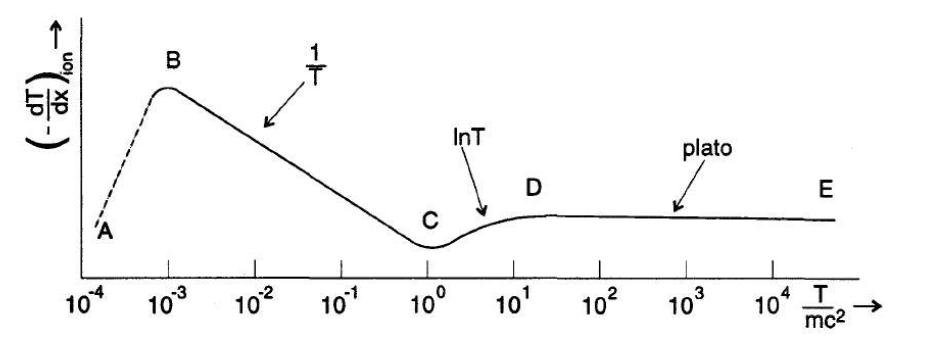
\includegraphics[width=1\textwidth]{JS2_bethe2.png}
	\captionof{figure}{Závislost $S_l$ na energii $T$ \label{obr:JS2_bethe2}}		
\end{center}

Závislost na Obr.\ref{obr:JS2_bethe2} si rozdělíme na čtyři části $AB, BC, CD $ a $DE$:
\begin{itemize}
	\item V oblasti $AB (0 - 1 ~\mathrm{MeV})$ Bethe-Blochova formule neplatí. děje se tak z následujících důvodů:
	\begin{itemize}
		\item Pro energie nižší než přibližně $1 ~\mathrm{MeV}$ nabitá částice začíná zachytávat a případně při následujících srážkách opět ztrácet elektrony (nábojová výměna). Následkem toho dochází ke změně náboje částice, záchytem elektronů se náboj částice neutralizuje.
		\item Rychlost částice je již srovnatelná s rychlostí atomárních elektronů na K-slupce, a proto se vnitřní atomární elektrony přestanou podílet na srážkách s letící nabitou částicí.
		\item Když je rychlost částice srovnatelná s rychlostí valenčních elektronů, začínají hrát úlohu ztráty pružným rozptylem s celými atomy, tzv. "jaderné brzdění". Přitom záchyt elektronů a jaderné brzdění hrají významnou roli hlavně při průchodu mnohonásobně nabitých iontů látkou.
	\end{itemize}
     \item V oblasti $BC (1 ~\mathrm{MeV} - 1000 ~\mathrm{MeV})$ Betheho formule platí. Ionizační ztráty klesají s rostoucí rychlostí (energií) částice jako
     \begin{equation}
     \left( - \dfrac{dE}{dx}\right)_{ion} \sim \dfrac{1}{v^2} \sim \dfrac{1}{T^2}
     \end{equation}
	Toto lze vysvětlit skutečností, že s klesající rychlostí částice se prodlužuje doba její interakce s atomárními elektrony.
	\item V oblasti $CD$ dosahují ionizační ztráty minima při energii přibližně $2mc^2$ ($\beta \gamma \sim 3- 4$) . Od této energie ionizační ztráty rostou jako $\ln T$. V této oblasti tedy Betheho formule platí, převažuje v ní logaritmický člen. Vzrůst $S_l$ lze vysvětlit lorentzovskou kontrakcí elektrického pole letící nabité částice, která díky tomu předá svou kinetickou energii i velmi vzdáleným elektronům (kolmá složka elektrického pole $E_\perp$ vzroste $\gamma$-krát).
	\item V oblasti $DE$ Betheho formule neplatí. Vzrůst ionizačních ztrát začne být při dalším růstu kinetické energie již omezen (\quotedblbase plato\textquotedblright). toto je způsobeno tím, že elektrické pole, kterým působí letící částice na vzdálený elektron, je zmenšováno elektrickým polem vyvolaným polarizovanými atomy látky (to je ale také vybuzeno letící nabitou částicí, resp. jejím elektrickým polem). Velikost této polarizace závisí na hustotě látky - zavádíme název \quotedblbase efekt hustoty\textquotedblright. Ten se uplatňuje při rychlostech částice $v > c/\sqrt{\epsilon}$, kde $\epsilon$ je dielektrická konstanta látky.
\end{itemize}	

Pro rozšíření platnosti Betheho formule i na oblasti $AB$ a $DE$ zavádíme korekční člen $U$ (pro oblast $AB$) a $\delta$ (pro oblast $DE$) zachycující efekt hustoty. Formule tak bude mít tvar
\begin{equation}
\left(- \dfrac{dE}{dx} \right)_{ion} = \left( \dfrac{1}{4 \pi \epsilon_0}\right)^2 \dfrac{4\pi  Z_{ion}^2 e^4}{m_e v^2}  \dfrac{Z}{A} \rho N_A \ln \left[ \left( \dfrac{2m_e v^2}{I}\right) - \dfrac{U}{2} - \dfrac{\delta}{2}\right] 
\end{equation}
Ionizační ztráty závisí na náboji a rychlosti letící nabité částice, ale nezávisí na její hmotnosti. Platí následující vztahy:
\begin{equation}
\left( - \dfrac{dE}{dx}\right) \sim \dfrac{1}{v^2} ,
\end{equation}
\begin{equation}
\left( - \dfrac{dE}{dx}\right) \sim Z_{ion}^2 ~~~~~~(\textit{Z těžkých iontů}),
\end{equation}
\begin{equation}
\left( - \dfrac{dE}{dx}\right) \sim Z ~~~~~~ (\textit{Z materiálu je dané počtem elektronů, větší Z, více elektronů})
\end{equation}

Pro střední budící potenciál $I$ (střední ionizační potenciál) používáme přibližnou hodnotu $I \approx 13,5 Z [\mathrm{eV}]$, kde $Z$ je atomové číslo, ačkoliv pro 
\begin{itemize}
     \item lehké prvky platí $I \approx 10 Z [\mathrm{eV}]$
     \item těžké prvky platí $ I \approx 15 Z [\mathrm{eV}]$.
\end{itemize}

\begin{center}
	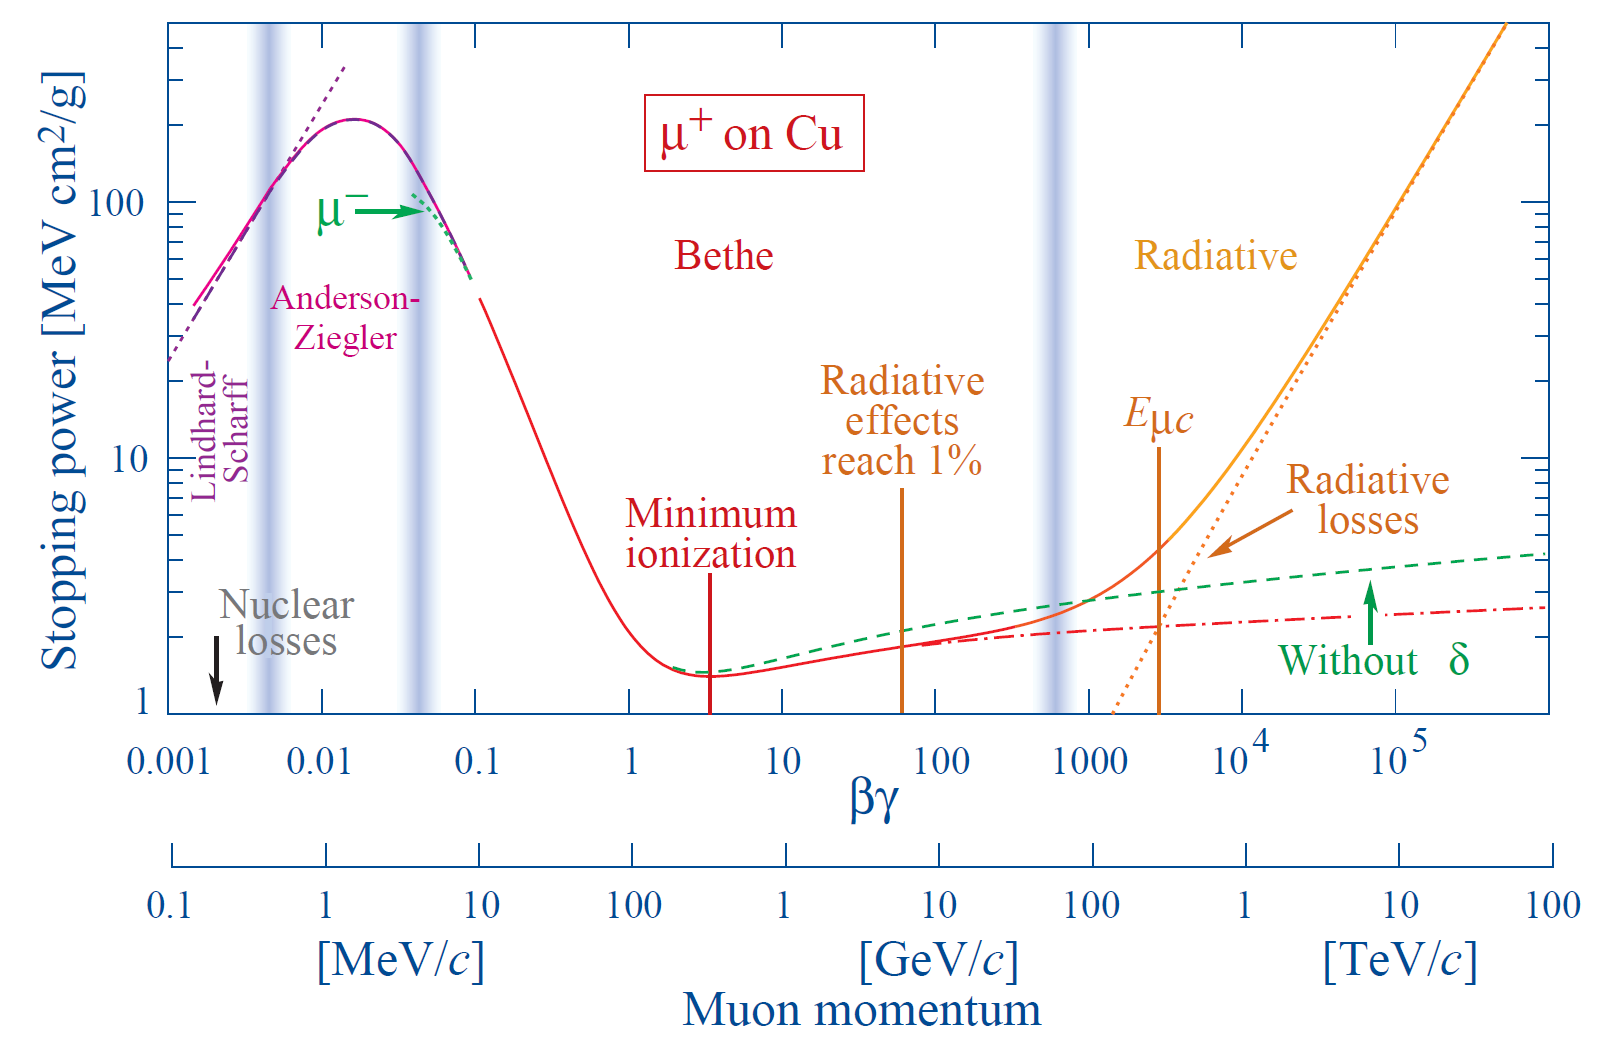
\includegraphics[width=1\textwidth]{JS2_bethe.png}
	\captionof{figure}{Závislost lineární brzdné schopnosti na kinetické energii částice pro miony v mědi \label{obr:JS2_bethe}}		
\end{center}

\subsection{Dosah těžkých nabitých částic}


\begin{center}
	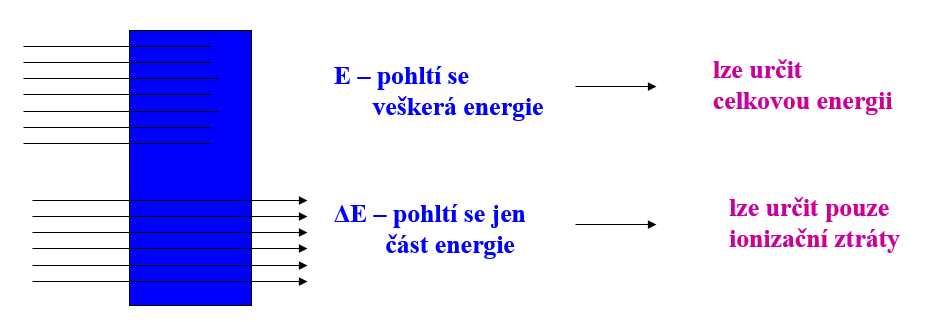
\includegraphics[width=0.8\textwidth]{JS2_pruchod.png}
	\captionof{figure}{U těžkých nabitých částic je jen slabě ovlivněn konec dráhy \label{obr:JS2_pruchod}}		
\end{center}


Matematicky je dosah definován pomocí vztahu (pro nerelativistický případ)
\begin{equation}
R = \int_{0}^{R} dx = \int_{0}^{R} \dfrac{dE}{dE} dx = \int_{T_0}^{0} \dfrac{dE}{\dfrac{dE}{dx}} = \int_{0}^{T_0} \dfrac{dE}{\left( - \dfrac{dE}{dx}\right) } = \int_{0}^{T_0} \dfrac{dE}{S_l} = \int_{0}^{T_0} T dT \cong T^2,
\end{equation}
kde $T_0$ je kinetická energie částice před dopadem do látky. V tomto vztahu jsme použili
\begin{equation}
\dfrac{dT}{dx} = \dfrac{dE}{dx} \sim \dfrac{1}{v^2} \sim \dfrac{1}{\dfrac{mv^2}{2}} = \dfrac{1}{T},
\end{equation}
kde
\begin{equation}
T = T_0 \left( 1 - \dfrac{x}{R}\right) .
\end{equation}
V relativistickém případě je $\beta$ $\rightarrow 1$ a máme konstantní ztráty energie. Minimální ionizace ($Z_{ion} = 1$), která je důležitá pro stavbu kalorimetrů je dána vztahem
\begin{equation}
\dfrac{dE}{d(\rho x)_{min}} = 1,5 ~\mathrm{MeV/(g/cm^2)}.
\end{equation}

 Použijeme-li ale pro $\left( - \dfrac{dT}{dx}\right) $ vztah pro Bethe-Blochovu formuli, dostaneme $R = \dfrac{m}{Z^2}f(v)$ , kde funkce $f(v)$ je pro konkrétní látku stejná pro všechny částice. Bethe-Blochova formule ale neplatí pro nízké energie částice, proto je třeba do uvedeného vztahu zavést korekci $C$, tedy
\begin{equation}
R = \dfrac{m}{Z^2} f(v) + C.
\end{equation}

Dosah těžkých nabitých částic je prakticky shodný s trajektorií částice, která je téměř přímková. Je to způsobeno tím, že těžké nabité částice nejsou významněji odchýleny žádnou srážkou, ke kterým navíc dochází ve všech směrech nezávisle. Závislost hustoty proudu těžkých částic v úzkém svazku na tloušťce absorbující vrstvy je vyobrazena na Obr.\ref{obr:JS2_prunik}.

\begin{center}
	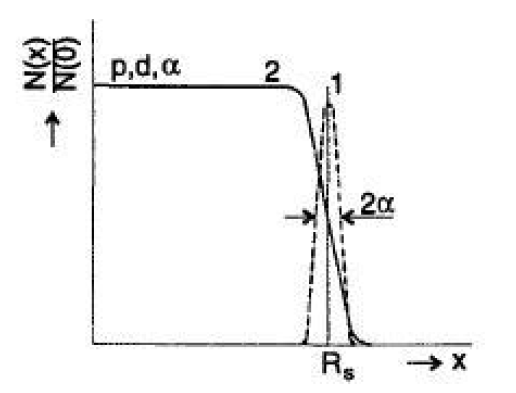
\includegraphics[width=0.6\textwidth]{JS2_prunik.png}
	\captionof{figure}{Počet částic v závislosti na hloubce průniku v látce \label{obr:JS2_prunik}}		
\end{center}

Počet částic nejprve zůstává téměř konstantní, poté začne prudce klesat k nule. Křivka označená 1 představuje diferenciální rozdělení dosahů, křivka 2 integrální rozdělení dosahů. Křivka 1 má Gaussovský tvar
\begin{equation}
\dfrac{dN}{dx} = \dfrac{N(0)}{\alpha \sqrt{x}} \exp \left[- \dfrac{(x-R_s)}{\alpha^2} \right] ,
\end{equation}
kde $\alpha$ je fluktuační parametr a charakterizuje šířku křivky; tento vztah vyjadřuje rozdělení dosahů kolem středního dosahu $R_s \equiv R$. Provedeme-li lineární extrapolaci v klesající části křivky 2, pak průsečík s osou $x$ určuje tzv. extrapolovaný dosah $R_e$. Mezi středním a extrapolovaným dosahem platí vztah 
\begin{equation}
R_e = R_s + \dfrac{1}{2} \alpha \sqrt{\pi}
\end{equation}
K určování dosahů v látce se ale často užívají empirické formule.

\begin{center}
	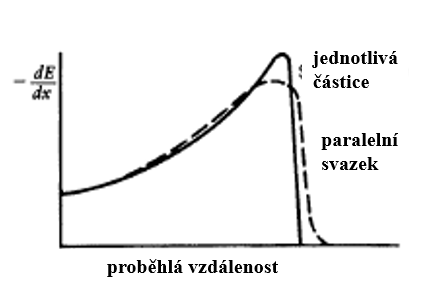
\includegraphics[width=0.6\textwidth]{JS2_ioni.png}
	\captionof{figure}{Průběh ionizačních ztrát pro jednotlivou částici a pro svazek částic se stejnou energií, tzv. Braggova křivka \label{obr:JS2_ioni}}		
\end{center}

\subsection{Braggova křivka}

Při průchodu těžkých nabitých částic látkou lze sledovat lineární ionizaci
\begin{equation}
\Delta N_l = \dfrac{\Delta N}{\Delta x},
\end{equation}
která je dána jako podíl počtu iontových párů $\Delta N$ vytvořených částicí na úseku dráhy $\Delta x$ a délky tohoto úseku. Závislost lineární ionizace na vzdálenosti se nazývá Braggovou křivkou. Ionizace roste od konce grafu k maximu a následně klesá směrem k menším délkám prolétnuté dráhy, tj. k vyšším energiím částice. V závěru života tedy částice ionizuje nejvíce - využívá se toho ve zdravotnictví při ozařování nádorů. Následný spád ionizačního účinku je způsobena tím, že těžká nabitá částice po svém zpomalení v látce redukuje svůj elektrický náboj nabráním elektronů.

\subsection{Chování štěpných fragmentů}

Těžké fragmenty produkované při štěpení (ať už indukovaném neutrony nebo spontánním) těžkých jader jsou energetické částice, jejichž vlastnosti se liší od těch do této chvíle probíraných. Jelikož odštěpky jsou na počátku zbaveny spousty elektronů, jejich velký efektivní náboj ústí ve specifické energetické ztráty, které jsou mnohem vyšší než u jiných těžkých nabitých částic. Navzdory tomu, že počáteční energie odštěpků je velmi vysoká, jejich dosah je přibližně polovina dosahu $\alpha$ částice s energií $5 ~\mathrm{MeV}$.
	
Podstatný rys štěpných fragmentů je fakt, že jejich energetické ztráty klesají s úbytkem energie v absorbátoru. Toto chování je v kontrastu s lehčími částicemi ($\alpha$ částice, protony) a je důsledkem stálého úbytku efektivního náboje neseného fragmentem.	

\subsection{Hadrony s vysokou energií - hadronová sprška}

Velká část energie je transformována jadernými reakcemi - tříštivé reakce produkce mezonů ($\pi^+ , \pi^- , \pi^0,...$). Důležitou charakteristikou je interakční délka. Kromě hadronové složky je přítomna i elektromagnetická složka daná hlavně rozpadem $\pi^0$, to se může rozpadat na dvě $\gamma$ částice, ty dále mohou produkovat pár $ e^+ + e^-$. Tím vzniká brzdné záření a tudíž elektromagnetická sprška.
\begin{equation}
\tau (\pi^0) = 8,4 \cdotp 10^{-17} ~\mathrm{s}, ~~~~~ \tau (\pi^+ \pi^-) = 2,6 \cdotp 10^{-8} ~\mathrm{s}, ~~~~~ \tau(\mu) = 2,2 \cdotp 10^{-6} ~\mathrm{s} ~~~~~~ c = 3 \cdotp 10^8 ~\mathrm{m/s}
\end{equation}

Poměr mezi elektromagnetickou a hadronovou složkou závisí na materiálu, odezva se nesmí měnit s energií. Velké množství neutronů vzniká vypařením z vysoce excitovaných jader. Energie, která je potřebná na jeden nukleon je $B \sim 8 ~\mathrm{MeV}$, rychle se ztrácí. 

\textbf{Kompenzační kalorimetry}: stejná odezva od elektromagnetické a hadronové složky, přesnost určení energie závisí na poměru těchto složek.


\section{Detektory těžkých nabitých částic}

Pro detekci těžkých nabitých částic potřebujeme dostatečně velké detektory, aby pohltily veškerou energii. Těžká nabitá částice začne okamžitě ionizovat materiál - většinou tedy vysoká účinnost.

Pro detekci můžeme použít:
\begin{itemize}
	\item Plynem plněné detektory
	\begin{itemize}
		\item Ionizační komory
		\item Proporcionální čítače
		\item Mnohodrátové komory
		\item Časově projekční komory
	\end{itemize}
	\item Scintilační detektory
	\item Polovodičové detektory
\end{itemize} 

\subsection{Scintilační detektory}

Odezva na těžké nabité částice:
\begin{itemize}
	\item začíná se projevovat nelinearita pro $L = f(E)$
	\item omezený počet scintilačních center $\rightarrow$ nasycení - část energie není konvertována 
	\item semiempirická Birksova rovnice: 
	\begin{equation}
	   \dfrac{dL}{dx} = \dfrac{A \dfrac{dE}{dx}}{1 + kB \dfrac{dE}{dx}}
	\end{equation}
	(hlavně pro organické scintilátory)
	\item Celkový světelný výstup $L$: $L = \int \left( \dfrac{dL}{dx}\right) dx$, kde $A$ je absolutní scintilační účinnost a $kB$ je parametr svazující hustotu ionizačních center s ionizací 
\end{itemize}
\begin{equation}
\dfrac{dE}{dx} \rightarrow 0 ~~ \Rightarrow ~~ \dfrac{dL}{dx} \sim \dfrac{dE}{dx}
\end{equation}
\begin{equation}
kB \rightarrow 0 ~~ \Rightarrow ~~ \dfrac{dL}{dx} \sim \dfrac{dE}{dx}
\end{equation}
\begin{equation}
kB \rightarrow \infty ~~ \Rightarrow ~~ \dfrac{dL}{dx} \sim \dfrac{A}{kB} \rightarrow 0
\end{equation}
\begin{equation}
\dfrac{dE}{dx} \rightarrow \infty ~~ \Rightarrow ~~ \dfrac{dL}{dx} \sim \dfrac{A}{kB}
\end{equation}
Z posledních dvou rovnic vyplývá, že saturace nastává, když:
\begin{equation}
L = \dfrac{A}{kB} R(E)
\end{equation}

\begin{center}
	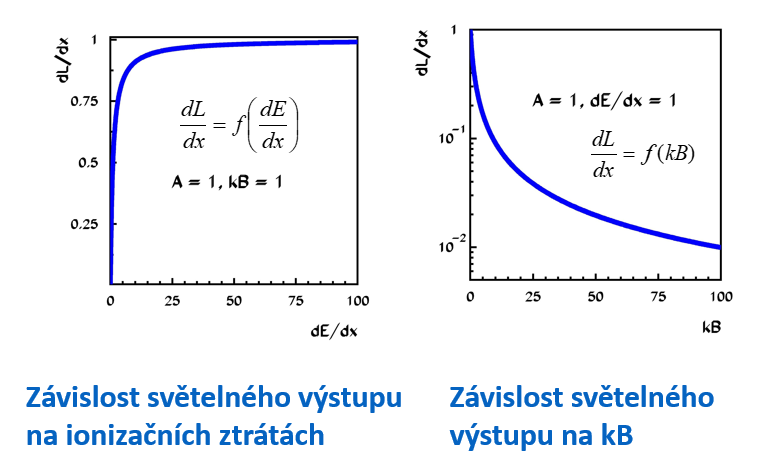
\includegraphics[width=0.8\textwidth]{JS2_scinti.png}
	\captionof{figure}{Závislost světelného výstupu na ionizačních ztrátách (vlevo) a na $kB$ (vpravo) \label{obr:JS2_scinti}}		
\end{center}

Různé ionty můžeme rozlišit pomocí analýzy tvaru pulsu:
\begin{itemize}
	\item krátká a dlouhá komponenta vysvěcování - vybíjení různých excitovaných stavů (v jakém poměru se budí závisí na ionizačních ztrátách)
	\item možnost použití dvou typů scintilátorů s různou dobou vysvěcování
	\item $\Delta E - E$ telescopy
\end{itemize}
\begin{equation}
\Delta E \approx \dfrac{Z^2}{E}
\end{equation}

\subsection{Hadronové kalorimetry}

Konec hadronové spršky nastává při $E \sim E_{THR} (\pi) \sim 100 ~\mathrm{MeV}$, což je práh produkce mezonů $\pi$. Energie má příčný tok energie a podélný tok energie - únik z detektoru. Chyba se potom skládá ze tří komponent:
\begin{itemize}
	\item statistické fluktuace: $\dfrac{\sigma _f}{E} \propto \dfrac{1}{\sqrt{E}}$
	\item detektorová - šumy, pedestaly: $\dfrac{\sigma _D}{E} \propto \dfrac{1}{E}$
	\item kalibrace - nelinearity fotonásobičů, nehomogenity: $\dfrac{\sigma _K}{E} \propto konst$
\end{itemize}

Detekuje se tak velké množství neutronů ($5\:neutronů/\mathrm{GeV}$) a jejich energie je $\sim 8 ~\mathrm{MeV}$.

\subsection{Kompenzační kalorimetr}

Větší odezva je pro částice elektromagnetické komponenty: $L_e/L_h = 1,1 - 1,35$. Pro aktivní a pasivní části kalorimetru je vhodné $L_e /L_h \approx 1$. Uran $238$ absorbuje pomalé neutrony, stínění měkkých fotonů vrstvou materiálu s malým $Z$ - absorpce fotonů ze záchytu neutronů pomocí atomů s velkým $Z$. Je zde možnost korekce při pozdějším zpracování díky využití informace o průběhu spršky. 

\section{Aplikace spektrometrie těžkých nabitých částic}

\begin{itemize}
	\item identifikace supertěžkých elementů pomocí sekvence rozpadů $\alpha$
	\item studium horké a husté hmoty pomocí spektrometrie nabitých částic
\end{itemize}

\subsection{Produkce supertěžkých prvků}
\begin{itemize}
\item Kapkový model:
\begin{itemize}
	\item s rostoucím protonovým číslem klesá stabilita
	\item s rostoucím protonovým číslem roste přebytek neutronů
\end{itemize}
\item Konkurence objemové energie (vazba silnou interakcí) a coulombovské energie. 
\item Existence \quotedblbase stabilnějších\textquotedblright ~supertěžkých elementů umožněna existencí magických čísel - slupkové struktury $\leftrightarrow$ slupkový model
\item ostrov stability - $Z = 114$ a $N = 184$ - závisí na tvaru potenciálu, značná neurčitost 
Problém:
\begin{itemize}
	\item velmi malé účinné průřezy
	\item produkce jen jednotlivých jader - nutná bezesporná identifikace
\end{itemize}
Energie:
\begin{itemize}
	\item dostatečná na překonání coulombovské bariéry
	\item co nejmenší, aby složené jádro vydrželo
\end{itemize}
Možnosti produkce:
\begin{itemize}
	\item neutronový záchyt - po $Z=100$ (pak dřívější rozpad než záchyt)
	\item reakce lehkého jádra na těžkém terči
	\item slučování těžkých jader \quotedblbase za studena\textquotedblright - projektil $A \sim 40$, $E_{EX} \sim 10 ~\mathrm{MeV}$
	\item slučování těžkých jader \quotedblbase ze horka\textquotedblright - použití $^{48}Ca$ ($Z = 20$), $E_{EX} \sim 40 ~\mathrm{MeV}$
\end{itemize}
Ve slučování těžkých jader \quotedblbase za studena\textquotedblright ~a \quotedblbase za horka\textquotedblright ~je rozdíl v projektilu a v excitační energii. Rozpad řadou rozpadů $\alpha$  $\rightarrow$ částice $\alpha$ nesou informaci o rozdílu energie jader.
\end{itemize}

\subsection{Detekce supertěžkých prvků v GSI Darmstadt}

\begin{itemize}
	\item Prvek $107 - 112$ - zařízení SHIP v GSI Darmstadt: slučovací reakce na jádrech Pb, Bi: využití separace, separace složeného jádra, implantace do aktivního objemu detektoru a identifikace pomocí řady rozpadů $\alpha$
	\item  Identifikace jednotlivých případů vzniku a rozpadu supertěžkého prvku:
	\begin{itemize}
		\item zachycení všech $\alpha$ částic ze sekvence rozpadů a určení jejich energie
		\item identifikace štěpení
	\end{itemize} 
    \item Rotující terč (Pb, Bi) - nízký bod tání
    \item intenzivní svazek - $10^{12}$ jader/s
    \item Výběr vzniklého složeného jádra:
    \begin{itemize}
    	\item Rychlostní filtr: $v_{CM} = \dfrac{m_p}{m_p + m_t}v_p$
    \end{itemize}
   \item Elektrické deflektory a dipólové magnety:
   \begin{itemize}
   	\item $F_{el} = q \cdotp E ~~~~~~~~ F_{mag} = q \cdotp v \cdotp B$
   \end{itemize}
    \item správný výběr $E$ a $B$ $\Rightarrow$ pro $v_{CM} $ je $F_{TOT} = F_{el} - F_{mag} = 0$
    \item Potlačení zbývajícího pozadí:
    \begin{itemize}
    	\item TOF spektrometr:
    	\begin{itemize}
    		\item Start - průchodové detektory, tenké uhlíkové fólie (produkce elektronů) a mikrokanálové destičky
    		\begin{itemize}
    			\item Efektivita $99,8 \%$, rozlišení $700 ~\mathrm{ps}$
    		\end{itemize}
    	     \item Stop - 16 křemíkových stripových detektorů, $\Delta E = 14 ~\mathrm{keV}$ pro $\alpha$ z $^{241}Am$
    	     \begin{itemize}
    	     	\item Pokrytí: 80 $\%$ z $2 \pi$
    	     \end{itemize}
    	\end{itemize}
    \end{itemize}
    \item HPGe detektory - fotony z vybíjení vybuzených jader
    \item Účinné průřezy až $\sim ~\mathrm{pb}$, jedno jádro za desítky dní
    \item Velmi intenzivní svazky po dobu měsíců
\end{itemize}

\begin{center}
	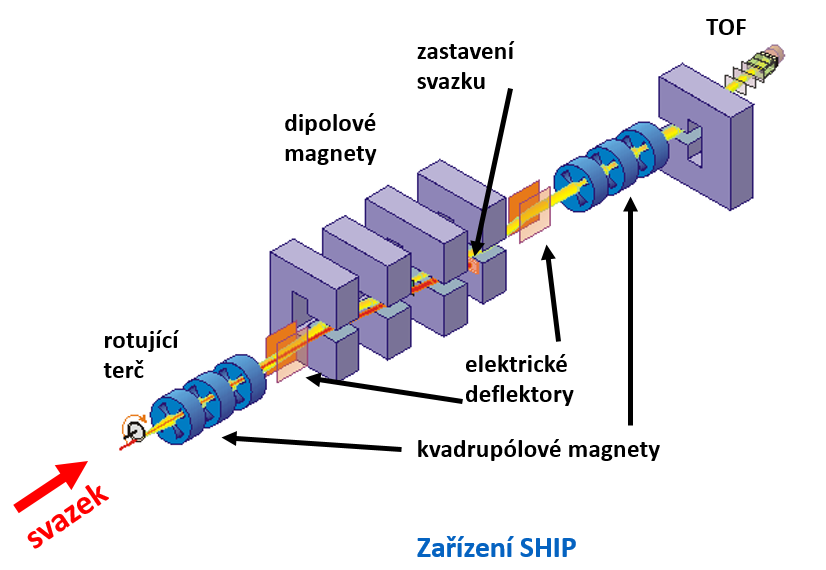
\includegraphics[width=0.9\textwidth]{JS2_SHIP.png}
	\captionof{figure}{Zařízení SHIP v GSI Darmstadt \label{obr:JS2_SHIP}}		
\end{center}

\textbf{Slučování při nízkých energiích}: objeveny následující prvky:
\begin{itemize}
	\item 107 ~~~ Bh ~~~ Bohrium
	\item 108 ~~~ Hs ~~~ Hassium
	\item 109 ~~~ Mt ~~~ Meitnerium
	\item 110 ~~~ Dm ~~~ Darmstadtiumu
	\item 111 ~~~ Rg ~~~ Roentgenium
	\item 112 ~~~ prokázán
\end{itemize}

Další - \textbf{slučování za vyšších energií}: (112, 113, 114, 115, 116, 118)

Problém:
\begin{itemize}
	\item nekončí to u známých izotopů (problém s navázáním)
	\item dost dlouhé poločasy rozpadu (problém s identifikací pomocí koincidencí)
\end{itemize}	

V r. 2006 - navázání - zdálo se to v pořádku

R. 2011 $\rightarrow$ $Z = 117$

R. 2015 - uznání $113, 115, 117, 118$

\subsection{Mapa supertěžkých prvků}

\begin{center}
	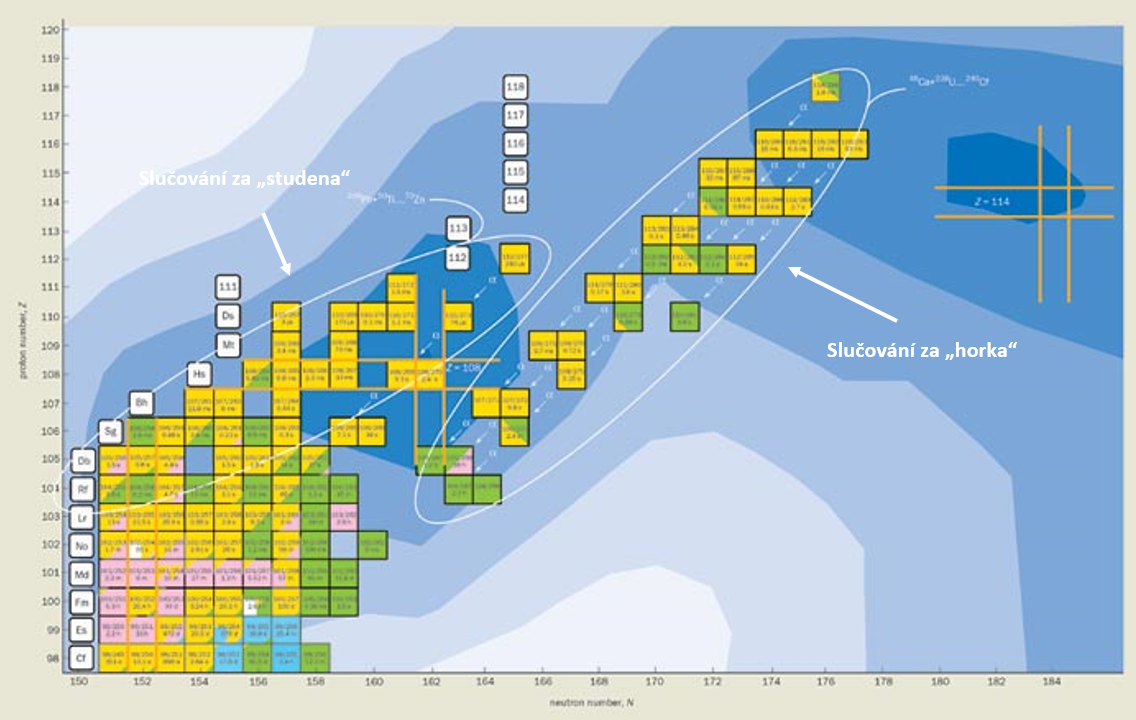
\includegraphics[width=0.9\textwidth]{JS2_mapa.png}
	\captionof{figure}{Mapa supertěžkých prvků \label{obr:JS2_mapa}}		
\end{center}

\subsection{Chemická analýza jednotlivých atomů}

\begin{itemize}
    \item Jádro se rozpadne dříve než vznikne další. Posledním prvkem zatím zkoumaných chemicky je 108 - Hassium. 
     \item Oxid hassičelý - HsO$_4$ $\rightarrow$ zkoumání těkavosti $\rightarrow$ oxidy X-čelé velmi těkavé.
     \item úzký kanálek s klesající teplotou od $-20\unit{^\circ C}$ do $- 170\unit{^\circ C}$ $\rightarrow$ čím těkavější tím dále se dostane než adsorbuje $\rightarrow$ je obklopen křemíkovým detektorem $\rightarrow$ detekují $\alpha$ ($4 \pi $ geometrie)
     \item Hs s $A \sim 288$ bude možná velmi stabilní
     \item nyní se chemicky zkoumá až po 113, 114 se začíná
 \end{itemize}

\subsection{Studium horké a husté hmoty pomocí produkce nabitých částic}

\begin{itemize}
	\item srážky relativistických těžkých iontů $\rightarrow$ velký počet produkovaných nabitých částic
	\item snaha o $ 4 \pi$ detektory nabitých částic
	\item příkladem je např. FOPI spektrometr v GSI Darmstadt
	\item určení teploty jaderné hmoty - průběh spektra
	\item určení tlaku - kolektivní toky částic 
	\begin{itemize}
		\item z tlaku a teploty $\Rightarrow$ určení stavové rovnice jaderné hmoty
	\end{itemize}

\begin{center}
	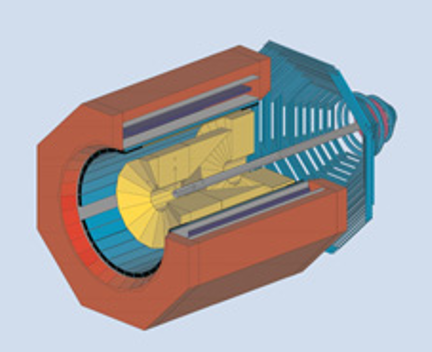
\includegraphics[width=0.5\textwidth]{JS2_FOPI.png}
	\captionof{figure}{Schéma FOPI spektrometru \label{obr:JS2_FOPI}}		
\end{center}

   \item zavedli jsme příčnou hmotnost $m_T$: $m_{T}^2 c^2 = m^2 c^2 + p_{x}^2 + p_{y}^2$
   \item a rapiditu $y$: $y = \dfrac{1}{2} \ln \left( \dfrac{\frac{E}{c} + p_z}{\frac{E}{c} - p_z} \right)$
   \item a tedy: $y = \dfrac{1}{2} \ln \left( \dfrac{mc + mv \cdotp \cos \theta}{mc - mv \cdotp \cos \theta}\right) = \dfrac{1}{2} \ln \left( \dfrac{1 + \beta \cdotp \cos \theta}{1 - \beta \cdotp \cos \theta}\right) $
   \item relativní rapidita: $Y_{REL} = (Y - Y_{PROJ}/2) /(Y_{PROJ}/2)$, kde $Y_{PROJ}$ je rapidita projektilu
   \item pro oblast terče platí: $Y_{REL} \rightarrow -1$, pro oblast srážky platí: $Y_{REL} \rightarrow 0$ a pro oblast projektilu platí: $Y_{REL} \rightarrow +1$
\end{itemize}

\subsection{Two Arm Photon Spectrometer}

\begin{itemize}
	\item detekuje kromě $\gamma$ taky nabité částice
	\item 384 BaF$_2$ detektorů s palstikovým vetem - rozlišení neutrálních a nabitých částic 
	\item součinnost s TOF stěnou z plastiku
	\item energie svazku $10 ~\mathrm{MeV} - 200 ~\mathrm{GeV}$ (GSI Darmstadt, KVI Groningen, GANIL Caen, CERN)
\end{itemize}

\subsection{Kolektivní toky nukleonů}

\begin{equation}
N = N_0 (1 + A \cdotp \cos \phi + B \cdotp \cos (2 \phi)),
\end{equation}
kde $A$ je velikost asymetrií v rovině srážky a $B$ je velikost asymetrií kolmo na ni (eliptický tok)

\begin{center}
	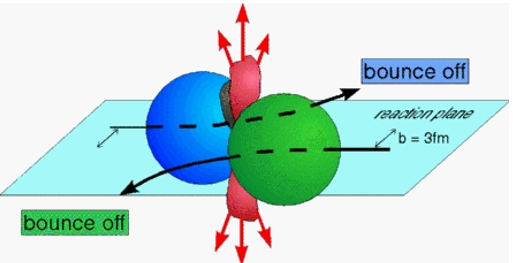
\includegraphics[width=0.5\textwidth]{JS2_kolekt.png}
	\captionof{figure}{Kolektivní toky nukleonů \label{obr:JS2_kolekt}}		
\end{center}

\begin{itemize}
	\item Realtivní rapidita:  $Y_{REL} = (Y - Y_{PROJ}/2) /(Y_{PROJ}/2)$, kde $Y_{PROJ}$ je rapidita projektilu
\end{itemize}

\begin{center}
	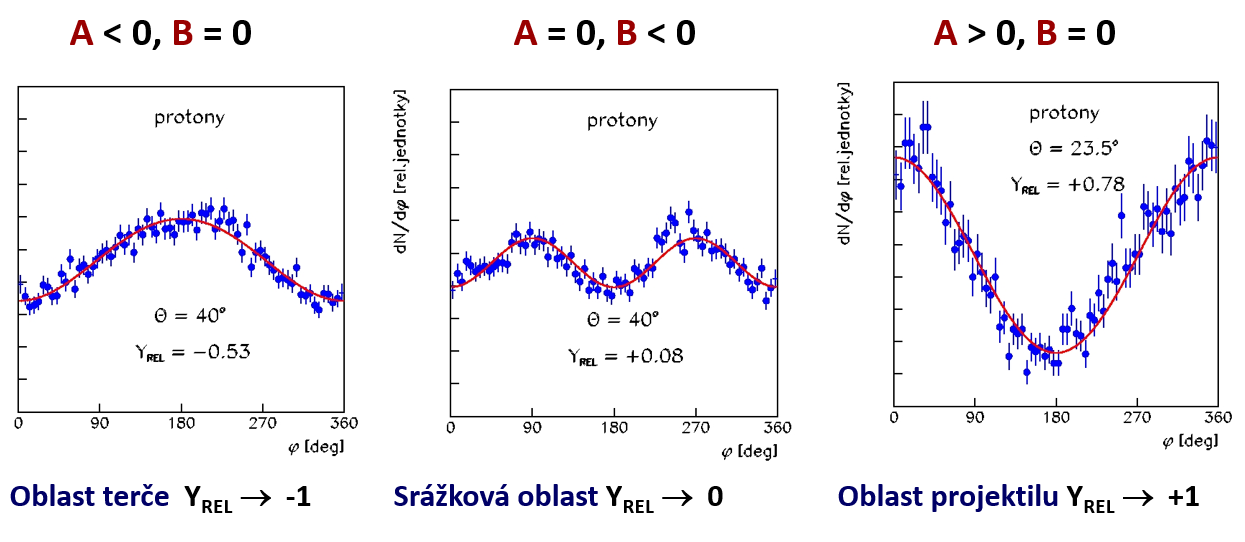
\includegraphics[width=0.5\textwidth]{JS2_kolekt2.png}
	\captionof{figure}{Relativní rapidita \label{obr:JS2_kolekt2}}		
\end{center}

\subsection{Závislost kolektivních toků na rapiditě}

\begin{itemize}
    \item Experimentální data - závislost velikosti kolektivního toku na počtu nukleonů - v souladu s hydrodynamickými modely
\end{itemize}

\begin{center}
	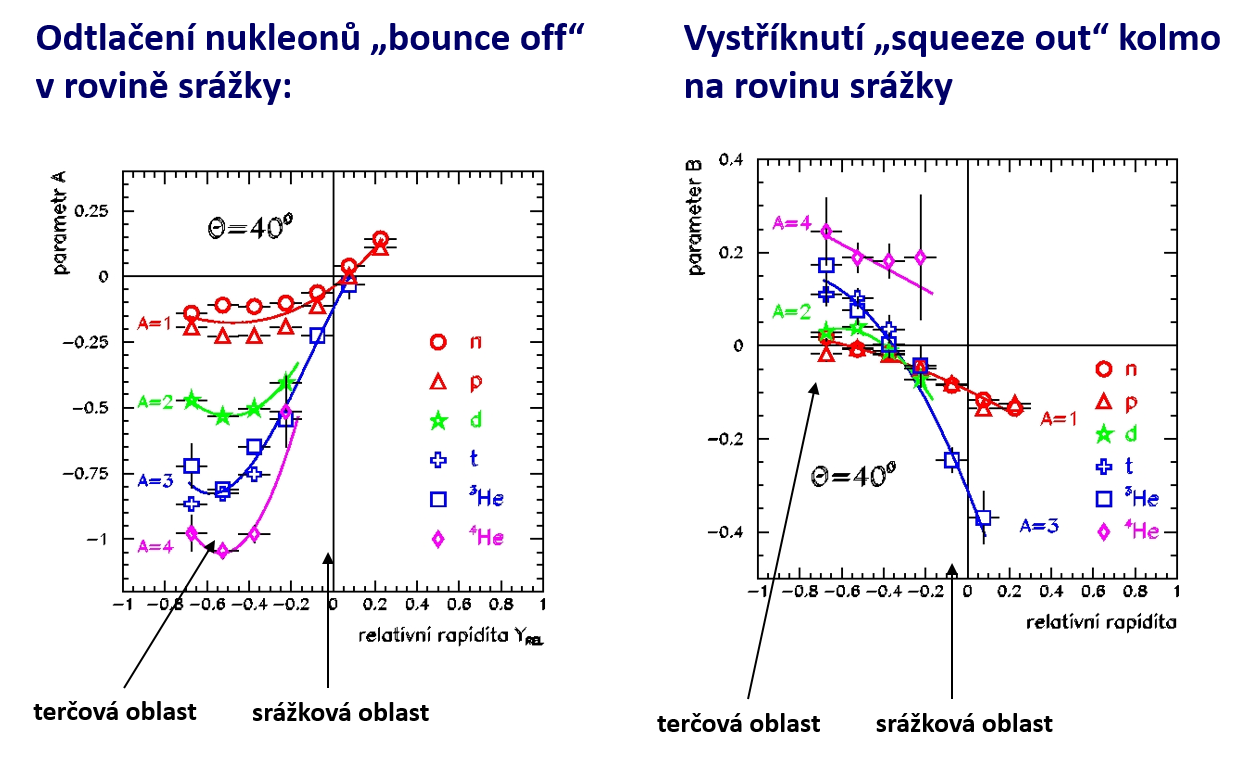
\includegraphics[width=0.5\textwidth]{JS2_kolekt3.png}
	\captionof{figure}{Závislost kolektivních toků na rapiditě \label{obr:JS2_kolekt3}}		
\end{center}

\subsection{Aplikace v materiálovém výzkumu - rozptyl, kanálování, reakce iontů, ...}

Ionty se využívají pro modifikaci a zkoumání struktury povrchových vrstev pevných materiálů. Využití urychlovačů iontů na urychlení na relativně nízké energie v řádu $\mathrm{keV}$ až $\mathrm{MeV}$. Spektrometry nabitých částic jsou často polovodičové křemíkové detektory.  

\subsection{Pružný rozptyl iontů}

\begin{itemize}
	\item RBS (Rutherford Backscattering Spectroscopy) - spektroskopie nabitých částic zpětně rozptýlených Rutherfordovým rozptylem - vrstvy od $\mathrm{nm}$ do $\mathrm{\mu m}$ - spektroskopie rozptýlených iontů polovodičovými detektory. Změna energie dána změnou hybnosti a ionizačními ztrátami - zjišťují se profily rozložení příměsí v materiálu - používá se pro těžká jádra.
	\item RBS channeling - kanálování nabitých částic - krystalické struktury - určení směrů význačných krystalových os a příměsí - natáčení krystalového vzorku
	\item ERDA (Elastic Recoil Detection Analysis) - detekce atomů vyražených iontů - spíše lehčí prvky, od vodíku až po dusík - lze tak i kontrolovaně měnit vlastnosti povrchů - studium obsahu vodíku v polymerech, spojení s měřením doby letu iontů
\end{itemize}

\begin{center}
	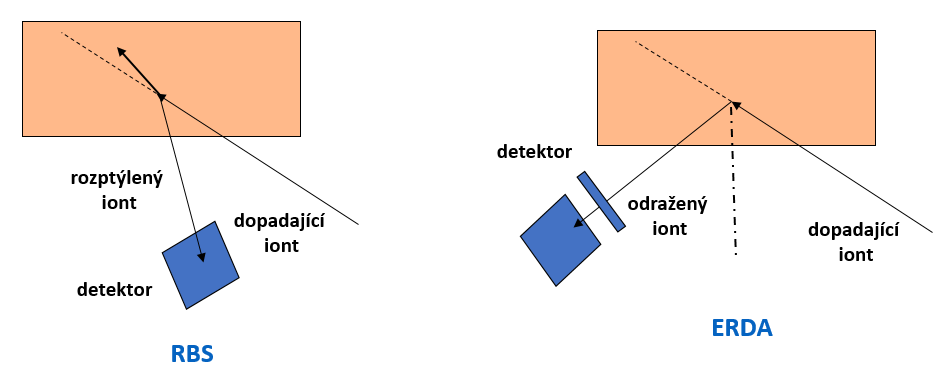
\includegraphics[width=1\textwidth]{JS2_RBS.png}
	\captionof{figure}{Vlevo je RBS, vpravo ERDA \label{obr:JS2_RBS}}		
\end{center}

\subsection{Reakce iontů s jádry}

\begin{itemize}
	\item PIGE (Particle Induced Gamma ray Emission)
	\item PIXE (Particle Induced Gamma ray Emission)
\end{itemize}

\subsection{Modifikace a opracování materiálů}

\begin{itemize}
	\item Iontová mikrosonda - velmi úzký intenzivní svazek iontů - použití  je skenování povrchů objektů s přesností v řádu mikrometrů
	\item Iontová implantace - modifikace povrchových vrstev materiálů
	\item Iontová litografie a obrábění iontovými svazky - příprava mikroelektronických a optoelektronických komponent a mikroskopických mechanických zařízení
	\item AMS - urychlovačová hmotnostní spektroskopie - příměsi prvků v koncentracích $10^{-15}$ - často pro uhlíkové datování
\end{itemize}

\end{document}